Firstly, we will go through the theoretical basis and its possible implementation
in the context of our task, after which, we will see the algorithm in action.

\subsection{Theoretical MinHashLSH}
\label{subsec:theoretical-minhashlsh}

The core of MinHashLSH algorithm is the utilization of two concepts: MinHash signatures and locality-sensitive hashing (LSH) to create and effective algorithm for detecting similar sets.
The first concept describes the process of hashing the dataset into a more manageable ``signature'' for each set.
While the latter describes how these ``signatures'' will be stored to achieve the expected result.

\subsubsection{Jaccard distance and Shingling}

Before performing any calculations to any data, we must convert the raw data into a distinguished vector before using any distance calculation between the two sets to check for their similarity.
Shingling performs this task by breaking down text data into smaller units to create ``shingles'' before hashing them into their representation in the form of a binary vector.

The Jaccard distance describes the similarity between two different sets and is represented by the following formula:
\begin{equation}
    \label{eq:equation}
    d_J(A, B) = \frac{|A \cup B| - |A \cap B|}{|A \cup B|} = 1 - J(A, B)
\end{equation}

With the result ranging from 0 to 1, we can determine whether the sets in question are related to each other or not for bucket assignment.

\subsubsection{MinHash Signature}

To determine if the pairs are similar or not, we need a way to convert the raw data into usable data for the algorithm to process.
In this case, MinHashing is used to perform this task.
The binary vector, created through a process of shingling, is converted into a signature vector.
Note that if these sets 2 are similar, their signature vector will also have some similarities, and these can be utilized by the algorithm to sort these sets into their suitable buckets.

\subsubsection{Locality Sensitive Hashing (LSH)}

The idea of LSH when dealing with the problem of finding similar pairs or sets is to maximize the probability of collision in a bucket due to that fact that the hash-code for these sets would be indifferent (if these sets are the same) and therefore they should be in the same bucket.
We can achieve this by breaking the hash-code down even more into subsequences of hash-code that have a higher chance of being similar, giving us a higher chance of finding similar pairs, improving the effectiveness of the algorithm at solving the problem.

\subsection{Optimized Manual Jaccard}
\label{subsec:optimized-manual-jaccard}
In the optimized manual Jaccard method, a broadcast join is used when one DataFrame is much smaller than the other, improving performance.
The Jaccard similarity is computed for each pair using a User-Defined Function (UDF).

Optimized Manual Jaccard: Instead of performing a complete cross-join, we use a broadcast join:
\begin{itemize}
    \item Apply the broadcast join between the smaller DataFrame and the larger one.
    \item Calculate Jaccard similarity using a UDF.
    \item Filter pairs based on the given similarity threshold.
\end{itemize}

With a manual method of calculating the Jaccard distance for each pair, we can utilize this function in our own Brute Force (BF) MinHashLSH algorithm

\subsection{Experimental Results}
\label{subsec:experimental-results2}
We evaluated both methods across various similarity thresholds.
Table~\ref{tab:comparison} presents the execution times and number of pairs processed for each method.

\begin{table}[h]
    \centering
    \caption{Comparison of MinHashLSH and Brute Force Across Thresholds}
    \begin{tabular}{|c|c|c|c|c|}
        \hline
        \textbf{Threshold} & \textbf{LSH Time (s)} & \textbf{BF Time (s)} & \textbf{LSH Pairs} & \textbf{BF Pairs} \\
        \hline
        0.0 & 33.83 & 13.21 & 218216 & 264628 \\
        0.1 & 36.09 & 13.30 & 218158 & 264520 \\
        0.2 & 35.37 & 12.55 & 202905 & 244672 \\
        0.3 & 21.93 & 13.08 & 91729  & 105487 \\
        0.4 & 12.46 & 13.04 & 8462   & 10113  \\
        0.5 & 11.19 & 13.19 & 132    & 223    \\
        0.6 & 10.79 & 23.84 & 2      & 3      \\
        0.7 & 10.98 & 21.78 & 0      & 0      \\
        0.8 & 10.89 & 24.46 & 0      & 0      \\
        0.9 & 9.25  & 23.88 & 0      & 0      \\
        1.0 & 10.77 & 21.68 & 0      & 0      \\
        \hline
    \end{tabular}
    \label{tab:comparison}
\end{table}

As you can refer from Table~\ref{tab:comparison} and subsequent graph, there is a distinct difference between both algorithms' performance.
For the traditional MinHashLSH implemented from the PySpark library, its runtime has a significant decrease as the threshold passes the 0.3 mark, taking up only one third of the time when compared to the runtime of a higher threshold.
Meanwhile, our Brute Force function while performing remarkably well at the first few increments of thresholds, it struggles to retain its performance when tasked to do such a task with a higher threshold.
All in all, despite having opposite trends, the BF function returns a higher efficiency with lower runtime and higher yield of frequent pairs.
This can be attributed to the fact that the BF function uses a different merging method with utilization of broadcast() function to optimize traffic, giving our BF function a better runtime on paper

\begin{figure}
    \label{fig:figure}
    \centering
    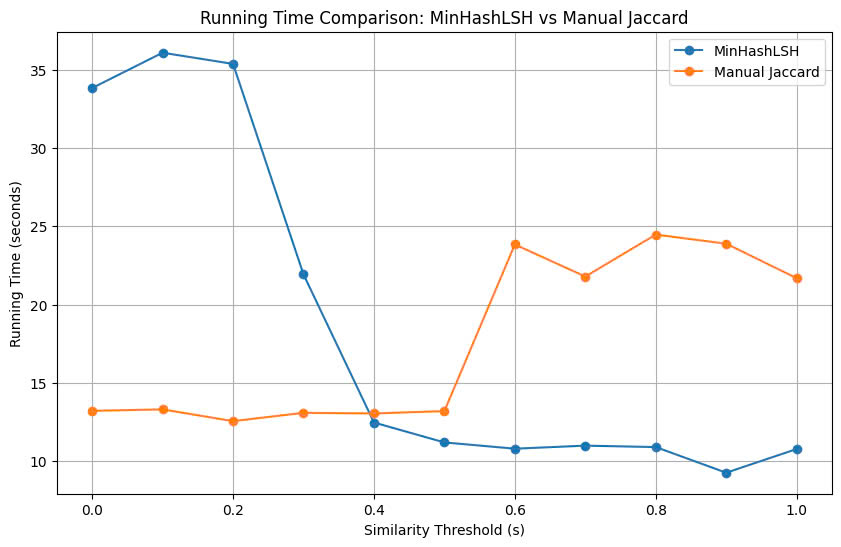
\includegraphics[width=\linewidth]{sections/Comparison_Graph}
    \begin{center}
        \caption{Comparison of Runtime with Incremental Thresholds}
    \end{center}
\end{figure}

\subsection{Conclusion}
\label{subsec:conclusion}
The optimized manual Jaccard method provides exact results but is computationally expensive, especially for large datasets.
In contrast, MinHashLSH is faster and works well for applications where approximate results are acceptable.
MinHashLSH is more suitable for performance-critical systems that require fast response times.